%%%%%%%%%%%%%%%%%%%%%%%%%%%%%%%%%%%%%%%%%%%%%%%%%%%%%%%%%%%%%%%%%%%%%%%%%%%%%%%%
%2345678901234567890123456789012345678901234567890123456789012345678901234567890
%        1         2         3         4         5         6         7         8

\documentclass[letterpaper, 10 pt, conference]{ieeeconf}  % Comment this line out
                                                          % if you need a4paper
%\documentclass[a4paper, 10pt, conference]{ieeeconf}      % Use this line for a4
                                                          % paper

\IEEEoverridecommandlockouts                              % This command is only
                                                          % needed if you want to
                                                          % use the \thanks command
\overrideIEEEmargins
% See the \addtolength command later in the file to balance the column lengths
% on the last page of the document



% The following packages can be found on http:\\www.ctan.org
\usepackage{graphicx} % for pdf, bitmapped graphics files
%\usepackage{epsfig} % for postscript graphics files
%\usepackage{mathptmx} % assumes new font selection scheme installed
%\usepackage{times} % assumes new font selection scheme installed
%\usepackage{amsmath} % assumes amsmath package installed
%\usepackage{amssymb}  % assumes amsmath package installed


\title{\LARGE \bf
CS 4758 Robot Learning: Beer Pong Butler
}

%\author{ \parbox{3 in}{\centering Huibert Kwakernaak*
%         \thanks{*Use the $\backslash$thanks command to put information here}\\
%         Faculty of Electrical Engineering, Mathematics and Computer Science\\
%         University of Twente\\
%         7500 AE Enschede, The Netherlands\\
%         {\tt\small h.kwakernaak@autsubmit.com}}
%         \hspace*{ 0.5 in}
%         \parbox{3 in}{ \centering Pradeep Misra**
%         \thanks{**The footnote marks may be inserted manually}\\
%        Department of Electrical Engineering \\
%         Wright State University\\
%         Dayton, OH 45435, USA\\
%         {\tt\small pmisra@cs.wright.edu}}
%}

\author{Kimberly Sheriff and Brian Toth}


\begin{document}



\maketitle
\thispagestyle{empty}
\pagestyle{empty}


%%%%%%%%%%%%%%%%%%%%%%%%%%%%%%%%%%%%%%%%%%%%%%%%%%%%%%%%%%%%%%%%%%%%%%%%%%%%%%%%
\begin{abstract}

This paper describes the application of the PR2 robot as a ''Beer Pong Butler", which will percieve  The PR2 will learn to identify a 

\end{abstract}


%%%%%%%%%%%%%%%%%%%%%%%%%%%%%%%%%%%%%%%%%%%%%%%%%%%%%%%%%%%%%%%%%%%%%%%%%%%%%%%%
\section{INTRODUCTION}

Beer pong, also known as Beirut, is a drinking game typically played at college parties, which involves two teams of two players each throwing ping pong balls across a table with the goal of sinking a ball into a cup of beer at the other end. Figure ~\ref{fig:pongtable}, shows the typical set up for a beer pong game. For our application, we will assume a game played with six cups on each side, which will be empty for our purposes. 

When a ball is successully thrown into a cup, that cup must be removed from the game. The beer pong butler will identify the cup that contains a ball and move that cup away from play.

\begin{figure}[thpb]
      \centering
	  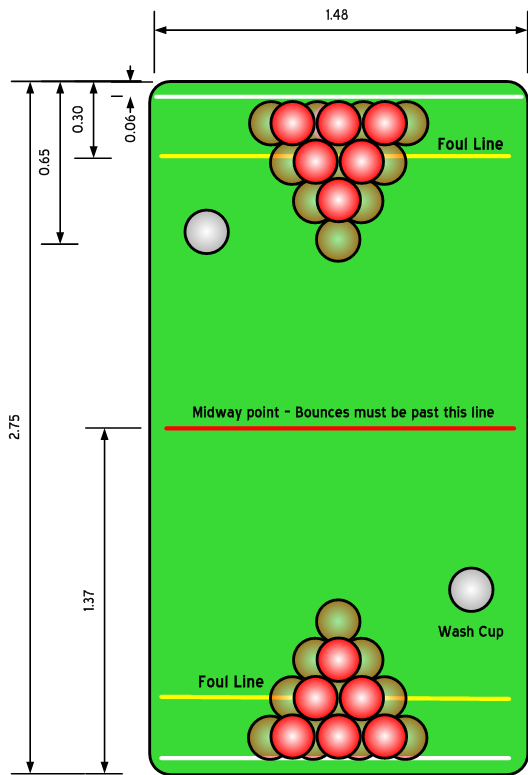
\includegraphics[scale =0.25]{pongtable}
      \caption{Typical beer pong setup.}
      \label{fig:pongtable}
\end{figure}


\section{Perception}

\subsection{Dataset}

Our data set is comprised of 51 images taken with the Kinnect. We label the cups one to six from left to right starting at the bottom left corner. The images were taken of various configurations of the cups, removing different sets of cups or no cups for each image. The angle and position of the Kinnect relative to the cup arrangement was also varied as was the lighting. Standard red plastic cups were used for all images. 

\subsection{Tabletop Detection}

Most of our effort was expended attempting to segment the tabletop from the objects on the table.  Although we were successful in doing so, the resulting pointcloud was not dense enough to actually determine which cup contained the ball.  To get around this, we are currently in the process of overlaying the pointcloud data on the rgb image data with mixed results.

\begin{figure}[thpb]
      \centering
	  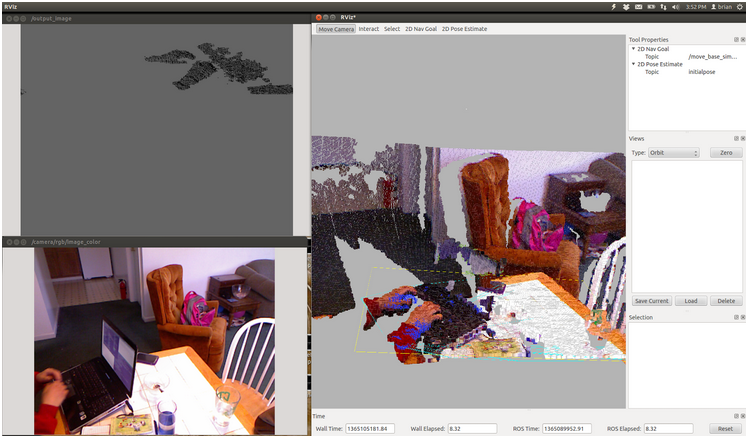
\includegraphics[width = 0.5\textwidth]{detect}
      \caption{Table top detection with pointcloud and rgb image data.}
      \label{fig:detect}
\end{figure}


\subsection{Cup Detection}

We considered a number of alternatives for using machine learning to bolster perception.  Although openCV’s Hough Circles do a good job of delimiting cups when properly tuned, as shown in Figure ~\ref{fig:positive}, they can perform erratically when the parameters are a bit off.  Slight changes in environment, lighting, height, or angle can result in incorrect or incomplete labeling of cups as seen in Figure ~\ref{fig:negative}.

\begin{figure}[thpb]
      \centering
	  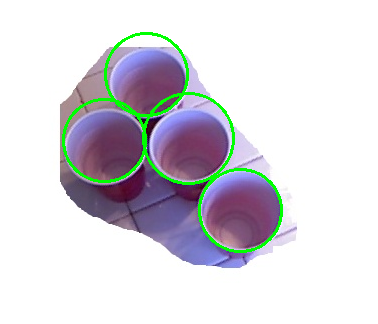
\includegraphics[scale =0.5]{4_cups}
      \caption{Positive example with all cups labeled correctly.}
      \label{fig:positive}
\end{figure}

\begin{figure}[thpb]
      \centering
	  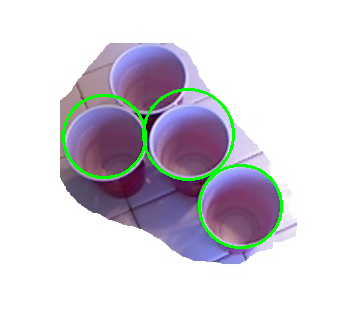
\includegraphics[scale =0.5]{4_cups_bad}
      \caption{Negative example with cup 6 not captured.}
      \label{fig:negative}
\end{figure}


Our first idea was to implement a combined HMM and SVM to determine whether we had properly identified the cups.  The problem naturally lends itself to an HMM, because there are a small number of discrete states (configurations of the cups), and the game naturally transitions from one state to another.  Even better, the transition probabilities are certainly not uniform and can be determined experimentally simply by throwing balls into cups.  Although we were very excited about this approach, it was abandoned due to time constraints.  Because each unique configuration would require a custom SVM to be trained, there would have to be 6+6+15+15+20+1+1= 64 different SVMs.  Gathering sufficient data to train and validate this many SVMs would not be practical.

Instead, we chose a solution that required only a single classifier.  By adding additional features to represent the implicit information in the HMM model, we plan to greatly reduce the number of training examples required.  The first six features represent the “best fit” that the Hough Circle detector can perform given the circles it finds.  Currently the assignment of numbers to cups is done by comparing to the initial 6 cup pyramid.  This makes the assumption that the robot does not significantly move during the course of the game; we are also pursuing an ‘absolute’ model based on coordinates.

The information from the “previous state” is incorporated in features 26-31.  Assuming the robot successfully removed a cup in the previous iteration and all of the circles were detected properly, this will match features 1-6 exactly.

The other features are currently experimental attempts to characterize a cup.  Our SVM is really doing double-duty; it requires both the detection of the correct number of cups in the correct relative positions and that the circles detected are actually cups.  At present we average the rbg values of the pixels within the cup-circles.

\section{Motion Planning}

We began by working with pick and place, but this algorithm does not work for our application because we are not picking up a stand alone object. We proceeded to investigate other motion planning techniques including an inverse kinematic solver. Given the x,y,z location of the center of the desired cup, our goal was to move the gripper three inches above that location. The three inches would allow room to rotate the gripper such that it is oriented downward into the cup. The gripper would then be move five inches downward so that the gripper is inside the cup near the center. The gripper would then spread, securing the cup. We would then raise the arm to remove that cup from the game.  This approach proved problematic due to sensitivity of the inverse kinematic solver. 



\begin{thebibliography}{99}

\bibitem{c1} G. O. Young, ÒSynthetic structure of industrial plastics (Book style with paper title and editor),Ó 	in Plastics, 2nd ed. vol. 3, J. Peters, Ed.  New York: McGraw-Hill, 1964, pp. 15Ð64.
\bibitem{c2} W.-K. Chen, Linear Networks and Systems (Book style).	Belmont, CA: Wadsworth, 1993, pp. 123Ð135.
\bibitem{c3} H. Poor, An Introduction to Signal Detection and Estimation.   New York: Springer-Verlag, 1985, ch. 4.
\bibitem{c4} B. Smith, ÒAn approach to graphs of linear forms (Unpublished work style),Ó unpublished.
\bibitem{c5} E. H. Miller, ÒA note on reflector arrays (Periodical styleÑAccepted for publication),Ó IEEE Trans. Antennas Propagat., to be publised.
\bibitem{c6} J. Wang, ÒFundamentals of erbium-doped fiber amplifiers arrays (Periodical styleÑSubmitted for publication),Ó IEEE J. Quantum Electron., submitted for publication.
\bibitem{c7} C. J. Kaufman, Rocky Mountain Research Lab., Boulder, CO, private communication, May 1995.
\bibitem{c8} Y. Yorozu, M. Hirano, K. Oka, and Y. Tagawa, ÒElectron spectroscopy studies on magneto-optical media and plastic substrate interfaces(Translation Journals style),Ó IEEE Transl. J. Magn.Jpn., vol. 2, Aug. 1987, pp. 740Ð741 [Dig. 9th Annu. Conf. Magnetics Japan, 1982, p. 301].
\bibitem{c9} M. Young, The Techincal Writers Handbook.  Mill Valley, CA: University Science, 1989.
\bibitem{c10} J. U. Duncombe, ÒInfrared navigationÑPart I: An assessment of feasibility (Periodical style),Ó IEEE Trans. Electron Devices, vol. ED-11, pp. 34Ð39, Jan. 1959.
\bibitem{c11} S. Chen, B. Mulgrew, and P. M. Grant, ÒA clustering technique for digital communications channel equalization using radial basis function networks,Ó IEEE Trans. Neural Networks, vol. 4, pp. 570Ð578, July 1993.
\bibitem{c12} R. W. Lucky, ÒAutomatic equalization for digital communication,Ó Bell Syst. Tech. J., vol. 44, no. 4, pp. 547Ð588, Apr. 1965.
\bibitem{c13} S. P. Bingulac, ÒOn the compatibility of adaptive controllers (Published Conference Proceedings style),Ó in Proc. 4th Annu. Allerton Conf. Circuits and Systems Theory, New York, 1994, pp. 8Ð16.
\bibitem{c14} G. R. Faulhaber, ÒDesign of service systems with priority reservation,Ó in Conf. Rec. 1995 IEEE Int. Conf. Communications, pp. 3Ð8.
\bibitem{c15} W. D. Doyle, ÒMagnetization reversal in films with biaxial anisotropy,Ó in 1987 Proc. INTERMAG Conf., pp. 2.2-1Ð2.2-6.
\bibitem{c16} G. W. Juette and L. E. Zeffanella, ÒRadio noise currents n short sections on bundle conductors (Presented Conference Paper style),Ó presented at the IEEE Summer power Meeting, Dallas, TX, June 22Ð27, 1990, Paper 90 SM 690-0 PWRS.
\bibitem{c17} J. G. Kreifeldt, ÒAn analysis of surface-detected EMG as an amplitude-modulated noise,Ó presented at the 1989 Int. Conf. Medicine and Biological Engineering, Chicago, IL.
\bibitem{c18} J. Williams, ÒNarrow-band analyzer (Thesis or Dissertation style),Ó Ph.D. dissertation, Dept. Elect. Eng., Harvard Univ., Cambridge, MA, 1993. 
\bibitem{c19} N. Kawasaki, ÒParametric study of thermal and chemical nonequilibrium nozzle flow,Ó M.S. thesis, Dept. Electron. Eng., Osaka Univ., Osaka, Japan, 1993.
\bibitem{c20} J. P. Wilkinson, ÒNonlinear resonant circuit devices (Patent style),Ó U.S. Patent 3 624 12, July 16, 1990. 






\end{thebibliography}




\end{document}
